\section{Construcción del índice: segunda parte}\label{sec:indice2}

\subsection{Inversión basada en merge}

Es inevitable citar a \citet[p. ~14]{Zobel06invertedfiles} (\citeyear{Zobel06invertedfiles}) y \citet[p.~238]{WittenMoffatBell99} (\citeyear{WittenMoffatBell99}), en donde encontramos que el método utilizado para llevar a cabo las operaciones descritas a continuación es un merge (mezcla) con la cantidad de documentos temporales que existan. Se muestra en la figura \ref{fig:indice2_1}.

\begin{figure}[!ht]
\centering
    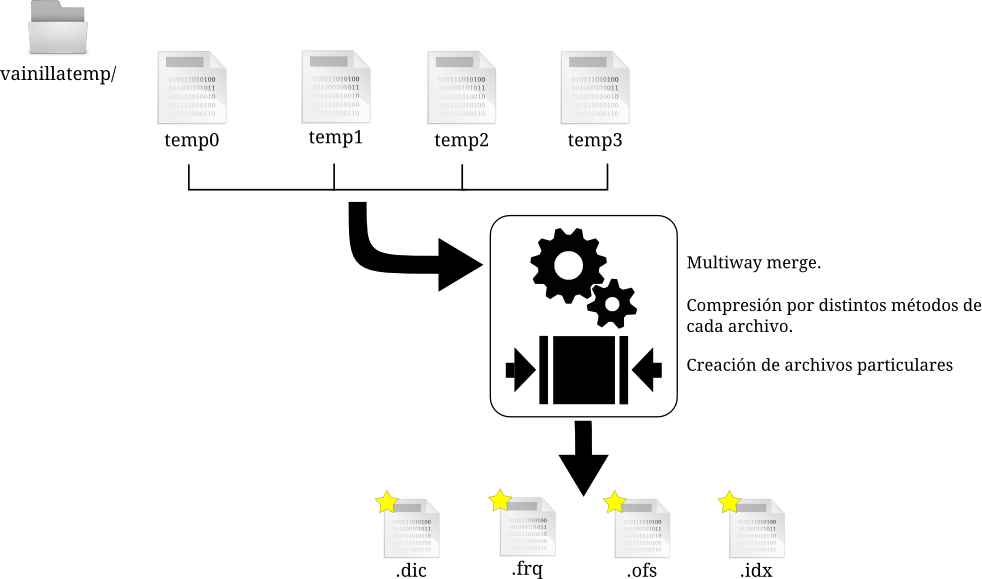
\includegraphics[scale=0.8]{./Images/indice2_1.png}
\caption{Multiway merge}
\label{fig:indice2_1}
\end{figure}


\subsection{Operatoria}

La segunda parte de la creación del índice parte del mergeo de todos los archivos temporales, y resulta en la creación de 4 archivos: diccionario, frecuencias, offsets e índice, a partir de ahora, archivos dic., frq., ofs. e .idx.

Al mergear registros del mismo término, se combinan las listas de docId's, frecuencias y posiciones de dicho término. Para cada término con sus datos obtenido, se realiza lo siguiente: -a

\begin {itemize}
\item En el archivo .dic se escribe el término codificado en LZW, avanza el puntero.

\item En el archivo .frq se escribe la suma de frecuencias del término en Rice Coding, avanza el puntero.

\item En el archivo índice, en la x posición del puntero, se escribe un bloque conteniendo dicho único término, y dentro de dicho bloque, cierta cantidad de fragmentos mayor o igual a 1. Cada fragmento va a guardar (por fragmento) cierta cantidad de posteos, siendo posteos lo siguiente: docIds que tengan el término (en forma de distancias), las frecuencias del término para doc en Rice Coding, y tantas listas de posiciones como docs codificadas en Pfor Delta. 

Hay que tener en cuenta que en cada fragmento se guarda hasta una cierta cantidad de posteos, siendo esta cantidad una constante definida. Nuestra constante definida es 128. Quiere decir que si el término está en más de 128 docs, cuando quiera guardar los datos sobre las ocurrencias en el doc 129, va a generar un fragmento nuevo. 

\item Luego de escribir en el .idx, en el archivo .ofs se escribe la posición actual del puntero al archivo índice en Rice Coding, y se avanzan ambos punteros (.idx y .ofs)

\end {itemize}
Cabe destacar lo siguiente como corolario:

Sea {\it t} un término que se encuentra en al menos un documento de la colección a indexar:

\begin {equation}
	\begin {aligned}
	.dic[x]&= t \\
	.frq[x]&= fg(t) \\
	.ofs[x]&= p \\
	.ind[p]&= bloque(t)
	\end {aligned}
\end {equation}

Tener en cuenta que un bloque en .idx se guarda la siguiente información para un solo término: docs en los que se encuentra, frecuencias en cada doc., posiciones en cada doc.


\begin{figure}[!ht]
\centering
    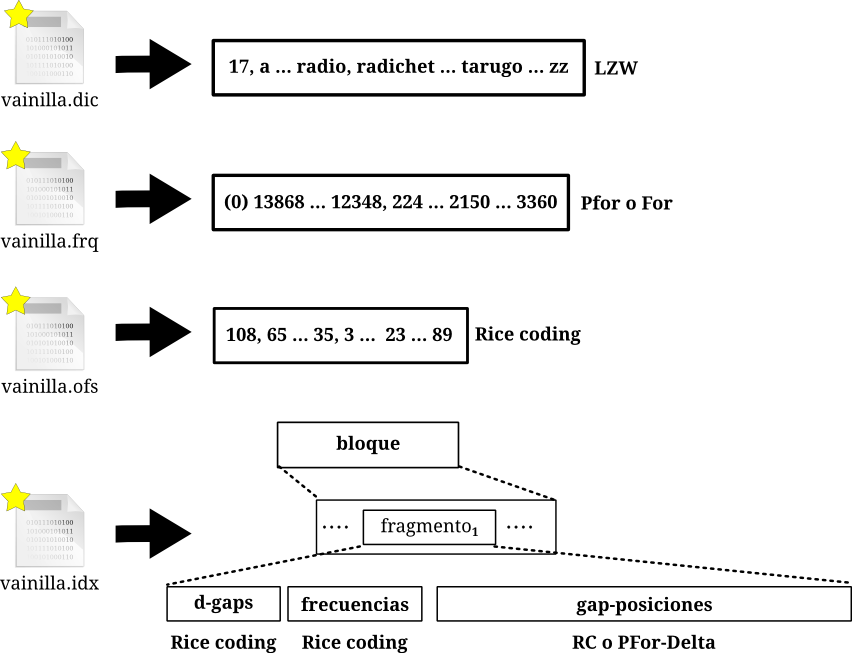
\includegraphics[scale=0.8]{./Images/indice2_2.png}
\caption{Archivos finales}
\label{fig:indice2_2}
\end{figure}



%Merge-based index construction is practical for collections of all sizes. In particular, it scales well and operates effectively in as little as 100MB of memory. In addition, disk space overheads can be restricted to a small fraction of the final index; only one parsing pass is required over the data; and the method extends naturally to phrase indexing. Finally, the compression techniques described in Section 8 can further reduce the cost of index construction by reducing the number of runs required.


%\begin{figure}[!h]
%\centering
%    
\includegraphics[scale=0.9]{./Images/vainillaDir.png}
%\caption{Ejemplo de directorio de trabajo}
%\label{fig:directorioTrabajo}
%\end{figure}


